% aus der Angabe kopiert:
%
% Dokumentation
% Dokumentieren und Beschreiben Sie: west, ninja, Kconfig,
% DTS, threads und message_queues (ca. 8 Seiten)
%
% zu allen genannten Punkten:
%
% * welches Problem löst es?
% * wie ist es umgesetzt?
% * wie unterscheidet es sich alternativen Lösungen?
%
% Der Code dokumentiert sich hoffentlich selbst, bzw. hat an kritischen Stellen
% Source Kommentare,
% d.h. nicht Teil der Dokumentation.
%
% Du solltest dich auf ca. 8 Seiten beschränken, d.h. auf die wichtigsten Dinge
% (was auch immer du für wichtig hältst und diese Auswahl ist Teil der Bewertung ;)


\section{Project Requirements}

The Project consists of the creation of a Processor which can receive data, then
encrypt or decrypt this data using AES-128 and then send it back via the
Serial-Interface.
\\
\\
The Processor should be developed using the
\href{https://docs.zephyrproject.org/2.0.0/boards/posix/native_posix/doc/index.html?highlight=native_posix}
{native\_posix-Board}.
Using the
\href{https://docs.zephyrproject.org/2.0.0/boards/posix/native_posix/doc/index.html?highlight=native_posix}
{native\_posix-Board} the Program can be compiled into a normal
executable which can be run on the Host-System (e.g. Linux).
\\
\\
The Serial-Interface should be implemented using the UART-Inteface which will connect to
/dev/pts/0 when the Board is started.
\\
\\
The Crypto-Processor should run using a predefined Statemachine and is to be
tested using a Python Unit-Test-Script.
\\
\\
The Cryptographic Operations (AES-128 Encryption and Decryption) should be implemented
using the Tinycrypt-Crypto-Device.

\begin{figure}[!ht]
	\begin{center}
		\includegraphics[width=\linewidth]{Statemachine.png}
		\caption{Statemachine}
	\end{center}
\end{figure}

\pagebreak

\section{Project Implementation Details}

The Project's Goal is to create a Encryption and Decrytion device which
doesn't need a lot of resources and can be easily accessed using UART.

\subsection{West}

West builds very efficiently because it especially targets devices with
less resources available.
\\
Because this project uses West, additional functionality can simply be added
by changing the Configuration-File.
\\
West also removes the need for a complex build-system but comes with the disadvantage
that a big workspace is needed and that a lot of overhead is generated during Compilation.

\subsection{Tinycrypt}

Tinycrypt enables devices with limited resources to encrypt and decrypt data
with a variety of Algorithms at a good pace because it is implemented using
Assembler.
\\
Tinycrypt's downside is that it needs it's memory setup in a particular manner
where the buffers are contingous.
\\
\\
Tinycrypt also only allows one Crypto-Operation at the same Time per device
which limits the scalabilty if no additional Hardware is provided.

\subsection{Program Implementation}

The Program is implemented using a Statemachine and seperate Message-Queues
per Thread which enables it to be modified very quickly.
\\
The Threads each have a dedicated task and complement each other, which creates
an efficient system as a whole, but require some baseline hardware to work.
\\
\\
The implementation on the
\href{https://docs.zephyrproject.org/2.0.0/boards/posix/native_posix/doc/index.html?highlight=native_posix}
{native\_posix-Board} has one big drawback which is that Interrupts cannot be
implemented.
This means the Program had to be developed using non-blocking Calls.
If the Program is to be implemented on a proper device these can be rewritten easily
using the equivalent blocking statements.

% \subsection{Program Implementation}
%
% Project Advantages:
% \begin{itemize}
% 	\item Easily modifiable\\
% 			The Project can be easily modified because of ``West``.\\
% 			The UART is also implemented in such a way that adding additional
% 			functionality is easy.\\
% 	\item Low Resource Intensity\\
% 			Because Zephyr only includes Dependencies it
% 			really needs and is developed to be efficient especially on limited Hardware\\
% 			The program was also developed in such a way that memory use is minimal.
% 	\item Project can be deployed to any Board which is already defined in Zephyr
% \end{itemize}
%
% Project Disadvantages:
% \begin{itemize}
% 	\item Project is rather complex because of the large Workspace and Build-Tools it needs
% 	\item Project takes long to build especially when the Dependencies are changed
% 	\item Currently only one Crypto-Action can take place at a time so it is
% 			hard to scale unless additional Hardware is provided.
% \end{itemize}

\pagebreak

\section{Used Technologies}

\subsection{Zephyr}

\href{https://zephyrproject.org/}
{Zephyr} is a small real-time operating system for embedded devices with constraints
on hardware resources which supports multiple different architectures
developed by
\href{https://www.linuxfoundation.org/}
{The Linux Foundation}.\\
Zephyr is released under the
\href{https://www.apache.org/licenses/LICENSE-2.0.html}
{Apache License 2.0}.
\\
\\
\href{https://docs.zephyrproject.org/2.4.0/index.html}
{Zephyr 2.4.0} was used for this Project.
It was installed for WSL2 on Windows 10 using the
\href{https://docs.zephyrproject.org/2.4.0/getting_started/index.html}
{official Getting-Started-Guide from Zephyr}

\subsubsection{KConfig}

\href{https://www.kernel.org/doc/html/latest/kbuild/kconfig-language.html}
{KConfig} is a configuration system originally developed for the Linux-Kernel
which can be used to enable or disable features or to select build-time-Options.

\subsubsection{Device Tree}

\href{https://docs.zephyrproject.org/2.0.0/guides/dts/index.html}
{The Device Tree} is a way of defining hardware and configuration
Information for Zephyr-Boards.
\\
It is used so Code can be dynamically included or excluded for
every Board without hard-coding every device into the OS.

\subsubsection{Threads}

A Thread is a sequence of instruction which can be run
independent of it's parent-process (the main-Thread in this case).
This allows the CPU to work on seperate Jobs simultaniously.

\subsubsection{Message-Queues}

Message Queues are FIFO-Buffers (First-In-First-Out-Buffers).
Buffers store data for later use and First-In-First-Out means
that the data which came in first comes out first.
FIFO-Buffers can deliver data between Threads in a safe manner.

\begin{figure}[!ht]
	\begin{center}
		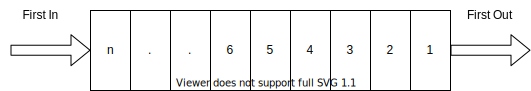
\includegraphics[width=0.4\linewidth]{Message_Queue.png}
		\caption{Message-Queue Example Diagram}
	\end{center}
\end{figure}

\pagebreak

\subsection{West}

\href{https://docs.zephyrproject.org/2.4.0/guides/west/index.html}
{West} is Zephyr's Meta-Tool, that means it uses other tools which
in turn build the actual application.
\href{https://docs.zephyrproject.org/2.4.0/guides/west/index.html}
{West} initializes, maintains and builds Zephyr-Workspaces
using
\href{https://ninja-build.org/manual.html}
{Ninja} and
\href{https://cmake.org/}
{CMake}.

\subsubsection{CMake}

\href{https://cmake.org/}
{CMake} is a Tool to automate Building, Testing and Packaging
in Software Projects.
\\
It can also generate Ninja Files for faster Building.

\subsubsection{Ninja}

\href{https://ninja-build.org/manual.html}
{Ninja} is a small build system that focusses on Speed.

\subsection{Linux Pseudo-Terminals}

\href{https://linux.die.net/man/7/pty}
{PTY's} also called
\href{https://linux.die.net/man/7/pty}
{Pseudo-Terminals} are bidirectional communication channels.
They enable Programs to transfer Data between one another
and appear as a normal File under /dev/pts/.

\subsection{Tinycrypt}

\href{https://01.org/tinycrypt}
{Tinycrypt} is a small footprint cryptography library written
in Assembler and implemented in Zephyr.
\\
It is developed and maintained by
\href{https://01.org/}
{Intel's Open Souce Technlolgy Center}.

\pagebreak

\section{Project Execution}

The Complete Codebase for the Project can be found on:
\href{https://github.com/davirieser/zephyr}
{Github}

\subsection{Block-Diagram}

The Serial-Crypto Processor is split into four Threads:
\begin{itemize}
	\item Main-Thread\\
		Responsible for starting the other Threads
	\item UART-In-Thread\\
		Responsible for incoming UART-Traffic and the Statemachine
	\item Processing Thread\\
		Responsible for Crypto-Operations
	\item UART-Out-Thread\\
		Responsible for outgoing UART-Traffic
\end{itemize}

\begin{figure}[!ht]
	\begin{center}
		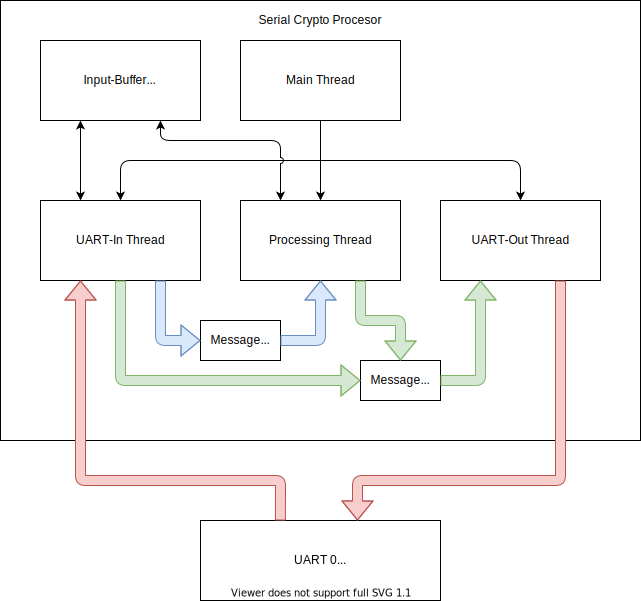
\includegraphics[width=0.75\linewidth]{Blockschaltbild.png}
		\caption{Serial Crypto Processor Block Diagram}
	\end{center}
\end{figure}

\pagebreak

\subsection{Build-Settings}

\begin{lstlisting}[caption=CMakelists.txt]
cmake_minimum_required(VERSION 3.13.1)

project(CRYPTO_UART)
find_package(Zephyr REQUIRED HINTS $ENV{ZEPHYR_BASE})

# Get all ".c"-Files in the src-Directory
FILE(GLOB MyCSources src/*.c)
target_sources(app PRIVATE ${MyCSources})
\end{lstlisting}

Get Dependencies for the Serial UART-Device and the Crypto-Device
according to
\href{https://docs.zephyrproject.org/2.4.0/reference/kconfig/index-all.html}
{Zephyr KConfig Documentation}

\begin{lstlisting}[caption=prj.conf]
# General config
CONFIG_NEWLIB_LIBC_NANO=n

# Configure Serial-Connection
CONFIG_SERIAL=y
CONFIG_UART_NATIVE_POSIX=y
CONFIG_NATIVE_UART_0_ON_OWN_PTY=y

# Configure Crypto Device Dependencies
CONFIG_CRYPTO=y
CONFIG_TINYCRYPT=y
CONFIG_TINYCRYPT_AES_CBC=y
CONFIG_CRYPTO_TINYCRYPT_SHIM=y
\end{lstlisting}

\begin{lstlisting}[caption=Makefile.posix]
# This makefile builds the sample for a POSIX system, like Linux

eventfd: src/main.c
	$(CC) $^ -o $@
\end{lstlisting}

\pagebreak

\subsection{Initialisation}

Initialisation consists of:
\begin{enumerate}
	\item Message-Queue Initialisation
	\item UART\_0 Initialisation
	\item Crypto-Device Initialisation
	\item Thread Initialisation
\end{enumerate}

\subsubsection{Message-Queue Initialisation}

The Message-Queues can be initialised using a Macro which
is already defined by Zephyr :
\\
\begin{lstlisting}[style=CStyle, caption=Message Queue Initialisation]
K_MSGQ_DEFINE(<Name>, <Data-Size>, <Queue-Length>, <Queue-Timeout>);
\end{lstlisting}
During Initialisation 2 Message-Queues are defined, one for
the UART-Out-Thread and one for the Processing-Thread:
\\
\begin{lstlisting}[style=CStyle]
// Create Message-Queues using Macros created by Zephyr
K_MSGQ_DEFINE(message_queue, sizeof(struct uart_message *), 20, 1);
K_MSGQ_DEFINE(crypto_queue, sizeof(char *), 20, 1);
\end{lstlisting}

\subsubsection{UART\_0 Initialisation}

The Initialisation of the UART\_0-Device for the native\_posix-Board
solely consists of getting the Handle for it :
\\
\begin{lstlisting}[style=CStyle,caption=UART 0 Initialisation]
// Get Handle to the UART_0-Device
uart_dev = device_get_binding(UART_DRV_NAME);

// Check that the UART_0-Device-Handle is correct
if (!uart_dev) {
	return -1;
}
\end{lstlisting}

\pagebreak

On the native\_posix-Board the Configuration of the Connection Parameters
for the UART can be ignored because Pseudo-Terminal are basically Buffers.
\\
On other Boards the correct Connection Parameters need to be set, otherwise
the Communication would not happen correctly:
\\
\begin{lstlisting}[style=CStyle, caption=UART-0 Configuration]
// Create UART_Config
const struct uart_config uart_cfg = {
	.baudrate = 115200,
	.parity = UART_CFG_PARITY_NONE,
	.stop_bits = UART_CFG_STOP_BITS_1,
	.data_bits = UART_CFG_DATA_BITS_8,
	.flow_ctrl = UART_CFG_FLOW_CTRL_NONE
};

// Configure UART_0-Device
if(!uart_configure(uart_dev, &uart_cfg)) {
	return -1;
}
\end{lstlisting}

\pagebreak

\subsubsection{Crypto-Device Initialisation}

The Initialisation of the Crypto-Device consists of getting the
Device-Handle and ensuring that the Hardware supports the
needed Capabilities for the Device:
\\
\begin{lstlisting}[style=CStyle,caption=Crypto-Device Initialisation]
// Get Handle to Crypto_Device
crypto_dev = device_get_binding(CRYPTO_DRV_NAME);

// Check that the Crypto-Device-Handle is correct
if (!crypto_dev) {
	return -1;
}

// Ensure that the Crypto-Device has the neccessary Hardware
if (validate_hw_compatibility(crypto_dev)) {
	return -1;
}
\end{lstlisting}

\begin{lstlisting}[style=CStyle,caption=Crypto Hardware Capability Check]
// Create global Struct for Crypto-Hardware-Capability-Flags
static uint32_t cap_flags;

// Ensure that the Device has the Capabilities to encrypt using Tinycrypt
int validate_hw_compatibility(const struct device *dev) {

    uint32_t flags = cipher_query_hwcaps(dev);
    if ((flags & CAP_RAW_KEY) == 0U) {
        return -1;
    }
    if ((flags & CAP_SYNC_OPS) == 0U) {
        return -1;
    }
    if ((flags & CAP_SEPARATE_IO_BUFS) == 0U) {
        return -1;
    }
    cap_flags = CAP_RAW_KEY | CAP_SYNC_OPS | CAP_SEPARATE_IO_BUFS;
	return 0;
}
\end{lstlisting}

\pagebreak

\subsubsection{Thread Initialisation}

Thread Initialisation happens in the Main-Thread.
The Threads are started one after another and their Handles are stored
in an Array:

\begin{lstlisting}[style=CStyle,caption=Thread Initialisation]
// Create Array for Thread-Handles
pthread_t threads[NUM_THREADS];

int ret, i;
pthread_attr_t attr[NUM_THREADS] = {};
void *(*thread_routines[])(void *) = {uart_in_thread,uart_out_thread,process_thread};

for (i = 0; i < NUM_THREADS; i++) {
	ret = pthread_create(&threads[i], &attr[i], thread_routines[i], INT_TO_POINTER(i));
	if (ret != 0) {
		return -1;
	}
}
\end{lstlisting}

\subsection{UART-In-Thread}

The UART-In-Thread works as the Brain of the whole Processor and is build
like a State-Machine:

\begin{lstlisting}[style=CStyle,caption=State Definitions]
// Declare Enums for State Machine
enum states{
	ST_INIT,ST_BUSY,ST_AVAIL,ST_ENCRYPT,ST_DECRYPT,
	ST_DLEN,ST_DATA,ST_KEY,ST_IV,ST_OP_SEL,ST_OP_KEY,
	ST_OP_IV,ST_OP_DECRYPT,ST_OP_ENCRYPT
};
enum operations{OP_INIT,OP_KEY,OP_IV,OP_ENCRYPT,OP_DECRYPT};
\end{lstlisting}

Upon Initialisation the Processor starts in the Initialisation-State which
is basically the IDLE-State:

\begin{lstlisting}
// Init Program States
static enum states prog_state = ST_INIT;
volatile static enum states processing_thread_state = ST_INIT;
static enum operations prog_operation = OP_INIT;
\end{lstlisting}

\pagebreak

From there on out the UART-In-Thread receives the Serial-Data and
handles them accordingly (Pseudo-Code) :

\begin{lstlisting}[style=CStyle,caption=State Machine Pseudo-Code]
// Run until the Stop-Flag is set
while (!stop_flag) {
	switch (prog_state) {
		case ST_INIT:
            // Wait for incoming Traffic
            if(!uart_poll_in(uart_dev,&uart_in)){
				// Handle Read
			}
	    case ST_DATA:
			// Read Data and set Buffer
	    case ST_IV:
			// Override IV with Buffer
	    case ST_KEY:
			// Override Key with Buffer
	    case ST_DECRYPT:
			// Decrypt Data and send it via the UART
	    case ST_ENCRYPT:
			// Encrypt Data and send it via the UART
	    default:
			// Reset Program State
	}
}
\end{lstlisting}

\pagebreak

\subsection{UART-Out-Thread}

The UART-Out-Thread handles the Processors Serial-Output and ensures
that each Message is sent one after another.
\\
For this a Struct was created so the data can be sent in a universal
Manner using a Pointer to a Sequence of Characters and the Length of
the String which lies at the Pointer's Location:

\begin{lstlisting}[style=CStyle,caption=Message Struct Definition]
struct uart_message{
	unsigned char * message;
	uint32_t len;
};
\end{lstlisting}

The UART-Out-Thread basically sits in an Endless-Loop and waits
for Messages to come in:

\begin{lstlisting}[style=CStyle,caption=UART Out Thread Pseudo-Code]
void * uart_out_thread(void * x) {

	int iLauf = 0;
	struct uart_message * message;

	// Run until the Stop-Flag is set
	while (!stop_flag) {
		// Block until Data is available
		if(!k_msgq_get(&message_queue,&message,K_NO_WAIT)) {
			// Send out Message Char by Char
			while(iLauf < (message->len)) {
				uart_poll_out(uart_dev,message->message[iLauf++]);
			}
			// Reset Counter
			iLauf = 0;
		}
	}
	return x;
}
\end{lstlisting}

\pagebreak

\subsection{Processing Thread}

The Processing Thread is the Worker of the Processor and handles the
Encryption and Decryption.
It is controlled using Commands which are send via a Message-Queue :

\begin{lstlisting}[style=CStyle,caption=Processing Thread Pseudo-Code]
unsigned char * message;
// Run until the Stop-Flag is set
while (!stop_flag) {
	if(!k_msgq_get(&crypto_queue,&message,K_NO_WAIT)) {
			switch (message[0]) {
				case ENCRYPT_CHAR:
					// Encrypt Buffer and send via UART
				case DECRYPT_CHAR:
					// Decrypt Buffer and send via UART
				case PROCESSING_CHAR:
					// Send "Processing Available"
				case WAIT_CHAR:
					sleep(10);
				default:
					break;
		}
	}
}
\end{lstlisting}

\subsection{Encryption and Decryption}

\subsubsection{Input and Output Buffers}

The Parameters for Encryption and Decrytion are stored in static global
Buffers so they can be accessed by all Threads when neccessary.

\begin{lstlisting}[style=CStyle,caption=Global Buffers for Encryption and Decryption]
static uint8_t * g_in_buffer;
static uint8_t * g_out_buffer;
// Create global Buffer-Length-Variable
static uint16_t buffer_length;

// Create contingous IV and Key with Default-Values "BBBBBBBBBBBBBBBB"
// This is Pseudo-Code
static uint8_t g_iv_key[AES_IV_LEN + AES_KEY_LEN];
memset(g_iv_key, 'B', AES_IV_LEN + AES_KEY_LEN);
\end{lstlisting}

To prevent Race-Conditions with these Buffers the UART-In-Thread can only
access the Buffers when the Processing-Thread is not using them.

\pagebreak

\subsubsection{Implmentation}

Encryption and Decryption are implemented in the same Funtion.
The caller can choose wheter to encrypt or decrypt using the
``en\_decrypt``-Argument:

\begin{lstlisting}[style=CStyle,caption=Encryption and Decryption Pseudo-Code]
uint32_t cbc_mode(const struct device *dev, uint8_t en_decrypt) {

	// Initialise Crypto Context using Key and Hardware Flags
	struct cipher_ctx ini = {
		.keylen = AES_KEY_LEN,
		.key.bit_stream = g_key,
		.flags = cap_flags,
	};
	// Create Buffers
	struct cipher_pkt buffers = {
		.in_buf = g_in_buffer,
		.in_len = in_buffer_len,
		.out_buf_max = out_buffer_len,
		.out_buf = g_out_buffer,
	};

	// Create Cipher Session which could be reused
	cipher_begin_session(crypto_dev,&ini,en_decrypt);

	// Execute Cipher Operation
	cipher_cbc_op(&ini,&buffers,);

	// Free Crypto Context
	cipher_free_session(dev, &ini);
}
\end{lstlisting}

After Encryption and Decrytion the Processing-Thread sends the Output-Buffer
to the UART-Out-Thread so it can be sent back via UART\_0.
Once the Output-Buffer is sent, the Processing-Thread forfeits access of
the Buffers so the UART-In-Thread can also modify them.

\pagebreak

\subsection{Unit-Tests}

To verify the functionality of the Crypto-Processor a simple Python Script
was provided.
\\
In this Python-File 6 Unit-Tests were definded:

\begin{itemize}
	\item If the Connection via UART works
	\item If the Crypto-Processor is available
	\item What is sent when the Crypto-Processor is busy
	\item What happens if someone tries to decode a faulty dataset
	\item A Test if a dataset is decrypted correctly using the standard Parameters
	\item A Decryption-Test using a custom Key and IV
\end{itemize}

All 6 Unit-Tests were passed by the Crypto-Processor.
